\chapter{Antecedentes y objetivos}
\label{cap:2-antecedentes}

\section{Antecedentes}

\subsection{La rotonda del Padre Anchieta}

La rotonda de Padre Anchieta (cuyo nombre real es «glorieta del Brasil») toma su nombre por la escultura, regalada por el pueblo brasileño, colocada en el centro de la rotonda en representación del beato José de Anchieta~\cite{gallo_glorieta_2013}.

La popularidad de la rotonda se explica por su posición estratégica, rodeada de viviendas, comercios, dos campus universitarios de la Universidad de La Laguna (Central y Anchieta), y por la cual pasa una de las principales autopistas de la isla, la TF-5; además de conectar otras cuatro vías: la carretera de la Esperanza (TF-24), la de Geneto (TF-263), la Av. Trinidad y la Av. Astrofísico. Sin embargo, los orígenes de la rotonda son considerablemente más humildes (véase la figura~\ref{fig:anchieta_ev}).

El tráfico que asume la rotonda es muy considerable, especialmente en horas punta, hasta tal punto en que se producen retenciones muy importantes y, en determinadas situaciones, un bloqueo total del tráfico, a veces durante horas (véase~\cite{gulesserian_vuelven_2018}, a modo de ejemplo). Las grandes cantidades de tráfico que absorbe la rotonda, y los bloqueos y ralentizaciones que se producen como consecuencia, tienden a afectar al tráfico de la TF-5, causando retenciones a la altura de la rotonda.

La optimización del tráfico en la rotonda se convierte, por tanto, en un asunto de primer orden respecto de la movilidad en la isla. La rotonda da una vía a los estudiantes tanto del norte como del sur que van a clase, a los trabajadores que se dirigen hacia La Laguna y hacia Santa Cruz; y en general a una gran cantidad de trayectos entre ambas ciudades y el norte de la isla que no puede dejarse desatendida.

\begin{figure}[h]
    \centering
    \begin{subfigure}[t]{.49\textwidth}
      \centering
      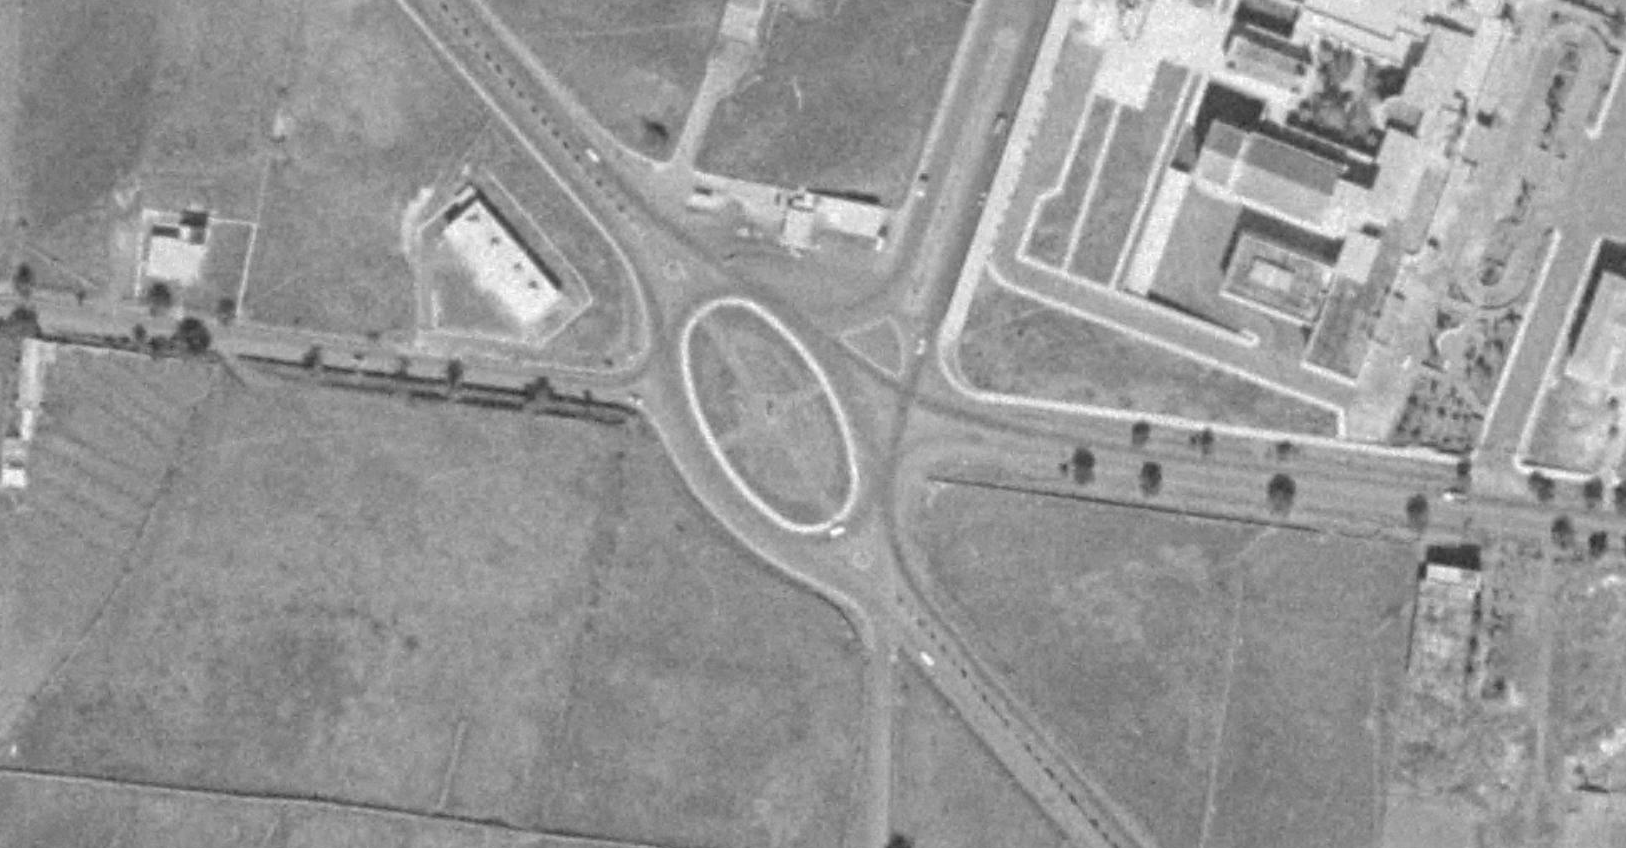
\includegraphics[width=\textwidth]{report/images/amp-anchieta-1964.png}
      \caption{1964}
      \label{fig:anchieta1964}
    \end{subfigure}
    \hfill
    \begin{subfigure}[t]{.49\textwidth}
      \centering
      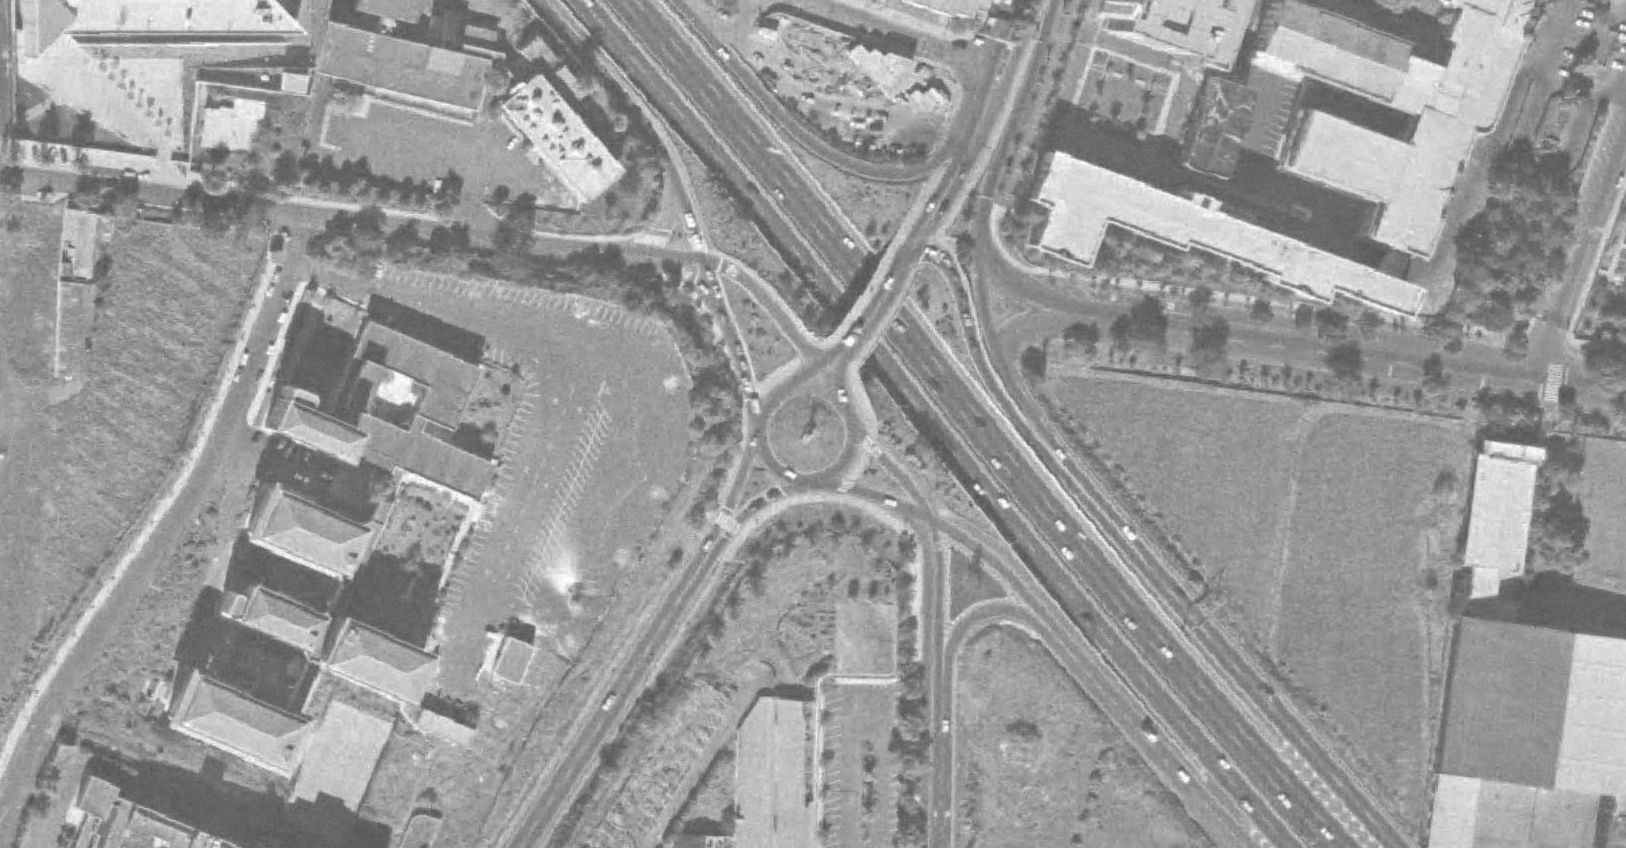
\includegraphics[width=\textwidth]{report/images/amp-anchieta-1994.png}
      \caption{1994}
      \label{fig:anchieta1994}
    \end{subfigure}
    \vspace{0.7cm}
    \begin{subfigure}[t]{.49\textwidth}
      \centering
      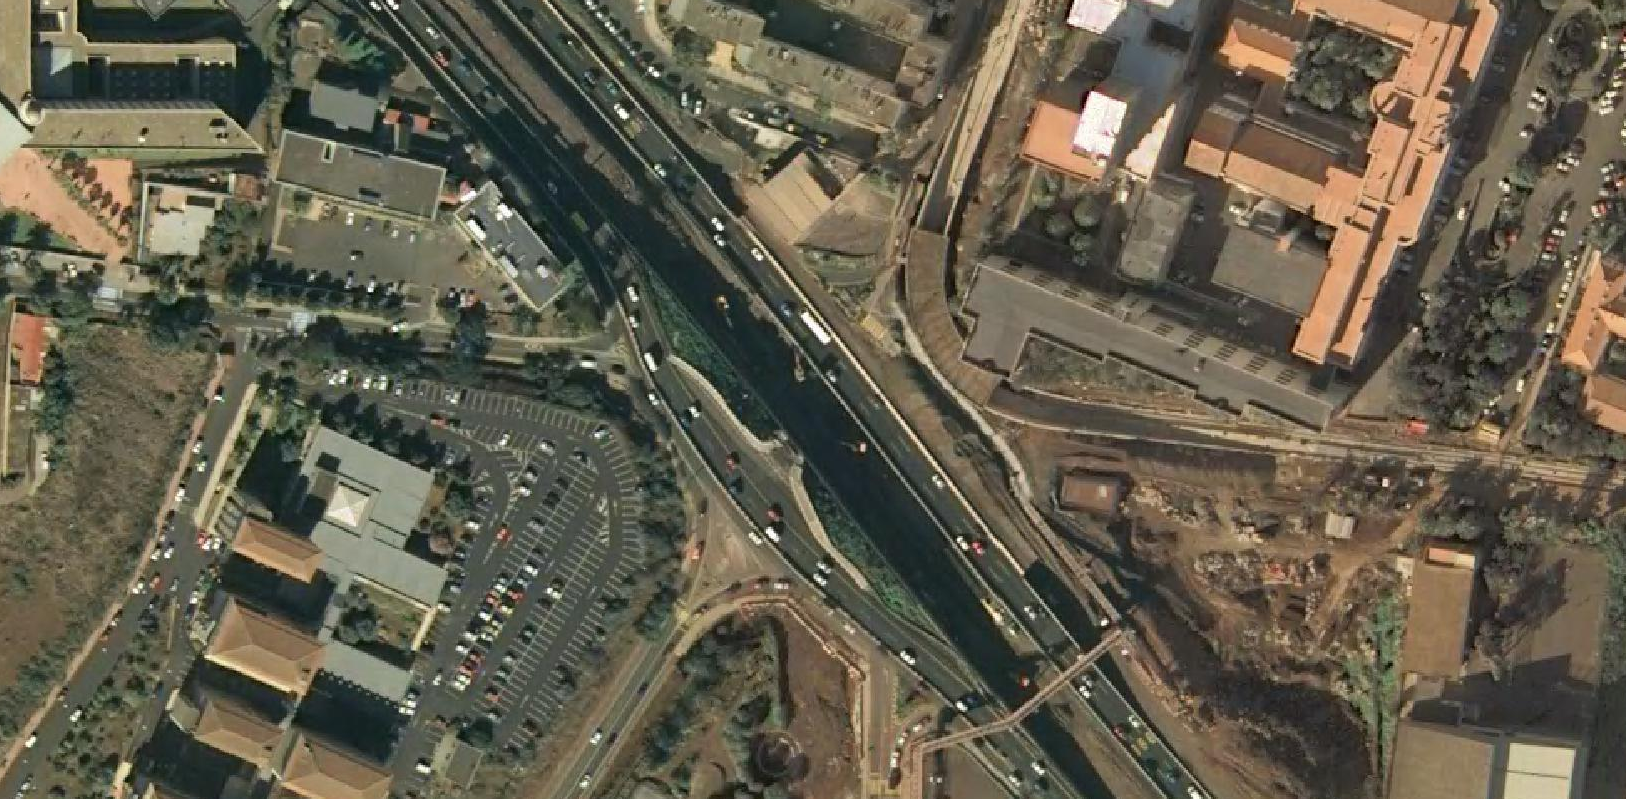
\includegraphics[width=\textwidth]{report/images/amp-anchieta-2006.png}
      \caption{2006 (en obras)}
      \label{fig:anchieta2006}
    \end{subfigure}
    \hfill
    \begin{subfigure}[t]{.49\textwidth}
      \centering
      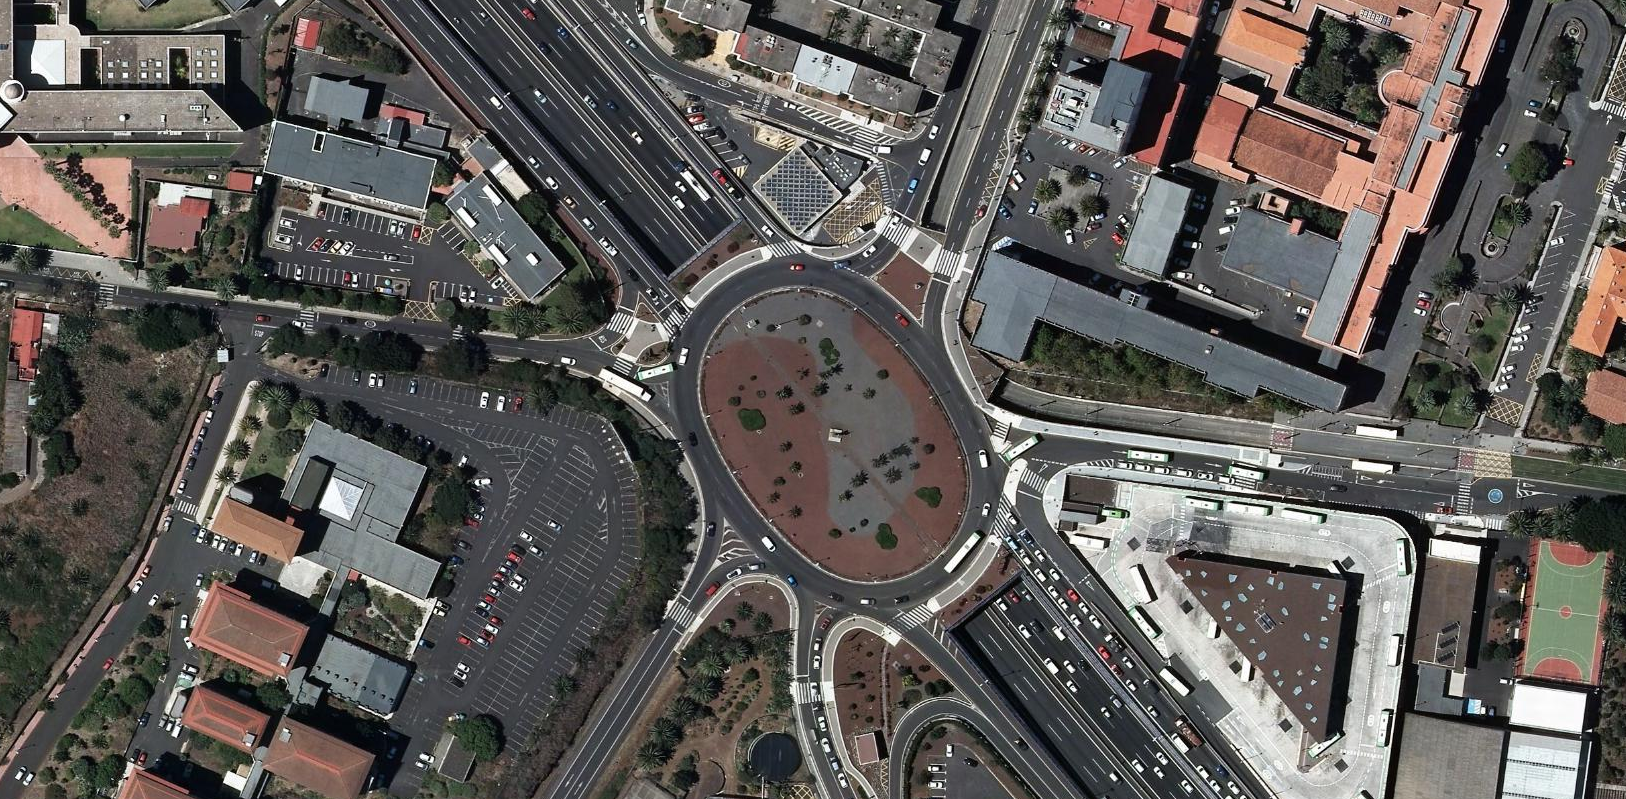
\includegraphics[width=\textwidth]{report/images/amp-anchieta-2019.png}
      \caption{2019}
      \label{fig:anchieta2019}
    \end{subfigure}
    \caption{Evolución de la rotonda de Padre Anchieta a lo largo de los años. Fotografías cortesía de GRAFCAN (\url{https://visor.grafcan.es/visorweb/})}
    \label{fig:anchieta_ev}
\end{figure}

\subsection{Mejoras propuestas}

Las autoridades de la isla no son ajenas al problema de tráfico que plantea de la rotonda. El Cabildo de Tenerife, organismo de cuya competencia depende la rotonda, y el Gobierno de Canarias, de cuya competencia depende la TF-5, han planteado varias medidas, de entre las cuales cabe mencionar:

\begin{itemize}
    \item El soterramiento de la TF-24 en dirección hacia Santa Cruz (a la espera de ejecutar el proyecto)~\cite{dia_cabildo_2019}.
    \item La construcción de una pasarela de peatones sobre la rotonda~\cite{rozas_pasarela_2019}.
    \item Potenciación del vehículo compartido y el transporte público: creación de carriles BUS-VAO en la TF-5~\cite{20minutos_gobierno_2019}.
    \item Propuestas para la construcción de nuevas líneas de tranvía~\cite{redaccion_de_eldiarioes_cabildo_2020}.
\end{itemize}

Sin embargo, todas las medidas mencionadas suponen un cargo importante al erario público, suponen una carga administrativa importante (por todos los procesos de licitación y control que han de realizarse), llevan mucho tiempo construirlas y mientras dure el proceso resultarán un incordio para los conductores y usuarios de la vía.

\section{Objetivos}

Con la elaboración de este proyecto lo que se propone es la instalación de semáforos en la rotonda, cuyas duraciones de fase han sido optimizadas mediante un algoritmo evolutivo, para comprobar si con la instalación de estos semáforos es posible mejorar la circulación del tráfico en función de determinados parámetros como la duración media de los trayectos de los vehículos, la velocidad media, la cantidad de vehículos que han logrado completar su trayecto en una hora, etc.


{\color{BurntOrange} HABLAR DEL TLSP!!!!!}


En comparación con las medidas antes mencionadas, la que se propone supone un coste considerablemente más bajo, no molestaría tanto a los conductores durante la instalación (la cual sería también mucho más corta y sencilla) y que plantea un problema muy interesante que podría ser reaprovechado para otras vías sin coste alguno (si ya tuvieran semáforos instalados).

Para llevar a cabo el proyecto, se han empleado principalmente dos herramientas.

\begin{itemize}
    \item La primera de ellas es SUMO~\cite{lopez_microscopic_2018}, un simulador de tráfico microscópico que nos permitirá evaluar cómo se comporta el tráfico en la rotonda de Padre Anchieta, con datos de tráfico provistos por el Cabildo de Tenerife.
    \item La segunda es Genetics.js~\cite{abrante_dorta_framework_2019}, una librería orientada a algoritmos evolutivos (en particular, algoritmos genéticos) programada en TypeScript.
\end{itemize}

\subsection{Trabajos previos relacionados}

El planteamiento aquí propuesto ya ha sido tratado desde distintas perspectivas por otros autores en los que se basa este TFG, de entre los que cabe resaltar a:

\begin{itemize}
    \item Segredo \textit{et al.}~\cite{segredo_optimising_2019}. El artículo versa sobre el TLSP y el empleo de varios optimizadores mono y multi-objetivos basados en la diversidad, por ser mucho más eficientes y, en consecuencia, ser capaces de lidiar con zonas significativamente más grandes de ciudades como Berlín, París, Estocolmo o Málaga, en vez de unas pocas intersecciones, llegando a simular casi 1000 de estas y más de 2600 vehículos.
    \item Sánchez \textit{et al.}~\cite{sanchez_applying_2008}. El artículo, de 2008, versa también sobre el TLSP pero aplicado a las Ramblas, en Santa Cruz de Tenerife. El autor, con la optimización propuesta de las duraciones de las fases de los semáforos, consigue mejoras notables en la circulación del tráfico.
    \item Dorta Acosta~\cite{dorta_acosta_simulacion_2019}. En este caso se trata de un TFG de un compañero de la Escuela, que versa sobre la instalación de semáforos inteligentes en la rotonda de Padre Anchieta.
\end{itemize}


{\color{BurntOrange} COMPLETAR CON ALGO MÁS? QUIZÁS PONER EN OTRO LUGAR ESTE APARTADO?}









